\documentclass[11pt,a4paper]{article}
\usepackage[margin=1in]{geometry}
\usepackage{amsmath,amssymb}
\usepackage{graphicx}
\usepackage{booktabs}
\usepackage{hyperref}
\usepackage{url}
\usepackage{xcolor}
\usepackage{enumitem}
\usepackage{natbib}
\usepackage{caption}
\usepackage{subcaption}
\usepackage{microtype}
\usepackage{float}

\hypersetup{
    colorlinks=true,
    linkcolor=blue,
    citecolor=blue,
    urlcolor=blue
}

\title{\textbf{Predicting Trump's Tweets from News Headlines:\\
A Comparative Study of Markov, N-gram, LoRA Fine-Tuning,\\
and Retrieval-Augmented Generation}}

\author{
  Rishabh Gulecha\\
  \texttt{rishabhgulecha28@gmail.com}\\[4pt]
  \small Code, data, logs, and trained model:\\
  \small \url{https://github.com/rishabh790453/trump-tweet-predictor}
}

\date{}

\begin{document}

\maketitle

\begin{abstract}
We study the problem of predicting Donald Trump's social media posts in response to contemporaneous news headlines, framing it as a conditional natural language generation task. We construct a large-scale dataset of 86,170 posts spanning Twitter and Truth Social (2009--2026) and semantically match each post to relevant news articles from a corpus of over 1.3 million New York Times and Guardian pieces. Four generation approaches are evaluated: (1) Markov chain and (2) N-gram statistical baselines operating purely on the tweet corpus, (3) a LoRA fine-tuned Llama 3 8B Instruct model trained on 25,000 news--post pairs with completion-only supervision, and (4) a retrieval-augmented generation (RAG) pipeline using FAISS-indexed embeddings over the matched dataset paired with a base Llama 3 8B Instruct model. Automatic evaluation across five diverse held-out examples spanning political, diplomatic, and domestic policy topics, scored using BLEU and ROUGE against verified ground-truth posts, shows the fine-tuned model and RAG achieving statistically similar performance (ROUGE-1: 0.154 vs.\ 0.153; BLEU-1: 0.055 vs.\ 0.056), both substantially outperforming statistical baselines. Qualitative analysis reveals a complementary failure mode: the fine-tuned model captures correct entities and topics but hallucinates URLs and structural artifacts, whereas RAG produces fluent, stylistically consistent outputs but generalizes less specifically to novel named entities. These findings motivate hybrid approaches and highlight the limits of surface metrics for evaluating stylistic generation.
\end{abstract}

\section{Introduction}

Presidential communication has been fundamentally reshaped by social media. Donald Trump's prolific use of Twitter (2009--2021) and Truth Social (2022--present) represents one of the most extensively studied corpora of political social media behavior \citep{bovet2019influence,wells2016trump}. His posts are characterized by a distinctive style: emphatic capitalization, punchy declarative sentences, direct attacks on named individuals and institutions, and rapid reactivity to news cycles.

The ability to predict such posts from contemporaneous news headlines has both scientific and practical implications. Scientifically, it tests whether language models can learn the mapping from world events to a specific individual's expressive register. Practically, researchers studying market reactions to presidential statements, political communication scholars, and policy analysts could benefit from a tool that anticipates the tone and content of politically consequential posts.

We formulate this as a \textit{news-conditioned tweet generation} task: given a set of news headlines published in the 48 hours preceding a known post, generate a post that resembles what Trump actually wrote. We compare four systems spanning the complexity spectrum from classical statistical models to large language models (LLMs) augmented with retrieval.

Our contributions are:
\begin{itemize}[noitemsep]
    \item A large-scale semantically-matched dataset of 65,733 news--tweet pairs, built from 86,170 posts and 1.3M news articles using sentence-level cosine similarity filtering.
    \item A systematic comparison of Markov chain, N-gram, LoRA fine-tuning, and RAG approaches on the same task, evaluated across five diverse held-out examples.
    \item Empirical evidence that fine-tuning and RAG achieve comparable average performance (ROUGE-1 $\approx$ 0.154), with complementary topic-dependent strengths that motivate hybrid architectures.
    \item An analysis of the limits of BLEU/ROUGE for evaluating stylistic text generation.
\end{itemize}

\section{Related Work}

\paragraph{Political text generation.}
Generating politically stylized text has attracted substantial attention since the availability of large presidential corpora. \citet{gpt2trump} demonstrated that GPT-2 fine-tuned on Trump's tweets produces stylistically recognizable outputs. \citet{rashkin2019towards} studied controllable political rhetoric generation. More recently, instruction-tuned LLMs have been prompted to impersonate political figures with varying fidelity \citep{argyle2023out}. \citet{herbold2024impersonate} showed that LLMs can impersonate politicians and public figures with varying fidelity, with persona-conditioned approaches outperforming generic prompting for idiosyncratic speakers. Our work extends this line by introducing news conditioning as the control signal and evaluating across four generation paradigms.

\paragraph{Retrieval-augmented generation.}
RAG \citep{lewis2020retrieval} augments LLM generation with retrieved documents at inference time, reducing hallucination and improving factual grounding. \citet{gupta2024ragsurvey} and \citet{gao2024retrievalaugmented} survey RAG systems extensively, finding that retrieval quality is the primary bottleneck — motivating our use of dense semantic retrieval over BM25 for stylistic examples. In our setting, retrieved (news, tweet) pairs serve as few-shot demonstrations that ground the model in Trump's actual vocabulary and reaction patterns.

\paragraph{Parameter-efficient fine-tuning.}
LoRA \citep{hu2022lora} reduces the computational cost of adapting billion-parameter models by injecting low-rank adapter matrices, training $<$1\% of parameters. \citet{dettmers2024qlora} extended this to 4-bit quantization, enabling fine-tuning on consumer hardware. We use standard bfloat16 LoRA on Apple Silicon (MPS), achieving comparable results without quantization given 32GB unified memory. Supervised fine-tuning with completion-only loss \citep{ouyang2022instructgpt} is critical to prevent prompt-leakage artifacts, a failure mode we encountered in preliminary experiments and document in Section~\ref{sec:failures}.

\paragraph{Presidential tweet analysis.}
A substantial body of work analyzes Trump's tweets for sentiment \citep{wang2017sentiment}, market impact \citep{bollen2011twitter,zhang2016predicting}, and political messaging strategy \citep{wells2016trump}. \citet{jiang2024trumppolls} simulate Trump-style public opinion in survey responses using LLMs, while \citet{schwager2026simulate} evaluate conditioned LLM comment prediction on real social media threads — both underscoring the broader interest in LLM-based social media simulation across the post-2020 political landscape. Our work is the first, to our knowledge, to directly predict tweet content from news headlines across multiple generation paradigms, jointly covering both platforms.

\section{Dataset Construction}

\subsection{Tweet Corpus}

We collected 86,170 posts from two platforms: 58,857 from Twitter (2009--2021) and 27,313 from Truth Social (2022--2026). The corpus covers Donald Trump's entire documented social media history across both platforms. Posts were filtered to remove retweets (RT prefix), replies (leading @mention), posts shorter than 30 characters after URL stripping, and posts longer than 400 characters. After filtering, 65,733 posts remained as candidates for training pair construction.

\subsection{News Corpus}

We assembled a news corpus of approximately 1.3 million articles: 1.27M from the New York Times (2009--2026) via the NYT Archive API and 32K from The Guardian, stored in a SQLite database. Articles are indexed by publication date, section, and headline text.

\subsection{Semantic News--Tweet Matching}

To construct training pairs, we match each post to relevant news articles using a 48-hour look-back window: for a post published on date $d$, we retrieve all articles published between $d-48h$ and $d$. Candidate pairs are scored by cosine similarity between sentence embeddings \citep{reimers2019sentence} of the article headline and the post, using the \texttt{all-MiniLM-L6-v2} model \citep{wang2020minilm}:

\begin{equation}
    \text{sim}(h, t) = \frac{\mathbf{e}_h \cdot \mathbf{e}_t}{\|\mathbf{e}_h\| \|\mathbf{e}_t\|}
\end{equation}

We retain pairs with $\text{sim} \geq 0.20$, keep the top-10 headlines per post, and discard posts where fewer than 3 headlines pass the threshold. This yields 65,733 training examples with an average similarity of $\overline{\text{sim}} = 0.339$, compared to $\approx 0.05$ for random pairings, confirming the pairs are semantically grounded. The dataset is split 90/10 into train (59,159) and validation (6,574) sets.

\section{Models}

\subsection{Baselines: Markov Chain and N-gram}

\paragraph{Markov Chain.}
A second-order Markov chain is trained on the full tweet corpus, building a transition table over 607,851 unique bigrams from 84,327 tweets. At generation time, the model is seeded with topic-relevant keywords extracted from the input headline and samples from the learned transition distribution until a stop condition is met. This model has no access to the news headline content beyond keyword seeding.

\paragraph{N-gram (Trigram).}
A trigram language model is similarly trained on the tweet corpus, with keyword-seeded generation. Both statistical baselines serve as lower bounds and represent the performance achievable from tweet-corpus statistics alone, without news-grounding.

\subsection{LoRA Fine-Tuned Llama 3 8B}

We fine-tune Meta's Llama 3 8B Instruct \citep{dubey2024llama} using Low-Rank Adaptation \citep{hu2022lora} on the semantically matched training set.

\paragraph{Training format.}
Each training example is formatted as a three-turn chat conversation: a \textsc{system} message instructing the model to respond as Trump, a \textsc{user} message containing the matched headlines, and an \textsc{assistant} message containing the corresponding post. We use TRL's \texttt{SFTTrainer} with \texttt{completion\_only\_loss=True}, which masks the system and user tokens from the loss computation so that gradients propagate \emph{only} from the assistant (post) tokens. This is a critical design choice: without this masking, the model learns to predict the repeated system prompt verbatim, causing prompt-leakage artifacts at inference time.

\paragraph{Hyperparameters.}
Training uses LoRA rank $r=16$ with $\alpha=32$, applied to all attention and MLP projection matrices ($q, k, v, o, \text{gate}, \text{up}, \text{down}$). We train for 1 epoch on 25,000 examples with effective batch size 32 (batch size 2, gradient accumulation 16), learning rate $2\times10^{-4}$ with cosine decay and 40 warmup steps, and sequence length 256. We use bfloat16 precision on Apple M5 (32GB unified memory) with the MPS backend. Training completes in approximately 17 hours (782 optimizer steps at $\sim$50s/step).

\paragraph{Hyperparameter choices.}
LoRA rank $r=16$ was chosen as a balance between adapter capacity and memory footprint; ranks of 8 and 32 were piloted and showed negligible validation loss difference ($<$0.05) at significantly higher training cost for $r=32$. We train for 1 epoch due to compute constraints (Apple M5, MPS backend, $\sim$50s/step). As shown in Figure~\ref{fig:training}, validation loss converges within the first epoch with no sign of overfitting, suggesting the primary stylistic features are captured within this budget; additional epochs may offer marginal gains at diminishing returns. Effective batch size 32 (micro-batch 2, gradient accumulation 16) is the largest that fits without OOM errors on 32GB. Learning rate $2\times10^{-4}$ follows standard LoRA practice \citep{hu2022lora}; cosine decay with 40 warmup steps prevents early instability.

\paragraph{Results.}
The model achieves validation loss 2.866 and mean token accuracy 45.4\% on post tokens only, measured on 2,500 held-out pairs. (Note: these metrics are not comparable to prior work that computed loss on the full sequence including prompt tokens, which inflates accuracy artificially.)

\subsection{Retrieval-Augmented Generation (RAG)}

The RAG pipeline uses a base (non-fine-tuned) Llama 3 8B Instruct model augmented with in-context retrieved examples. At index build time, all 65,733 training pairs are embedded using \texttt{all-MiniLM-L6-v2} and stored in a FAISS \texttt{IndexFlatIP} (inner-product / cosine similarity) index. At inference time, the input headlines are embedded and the top-$k$ most similar (headline, tweet) pairs are retrieved and inserted as few-shot examples in the prompt.

The prompt structure is: a system message defining the Trump persona, followed by $k$ retrieved (headline, tweet) examples as \texttt{user}/\texttt{assistant} turns, followed by the query headlines as the final user turn. The model then generates a new tweet. We use $k=5$ retrieved examples and generate with temperature 0.85.

The RAG approach requires no fine-tuning and benefits from real Trump vocabulary and reaction patterns at inference time, at the cost of prompt length.

\section{Evaluation}

\subsection{Experimental Setup}

We evaluate all models on five held-out examples drawn from verified Trump posts published in April 2026, covering diverse topics: (1) NYC luxury tax policy (Mamdani), (2) Lebanon--Israel ceasefire negotiations, (3) Strait of Hormuz / China diplomacy, (4) White House ballroom legal challenge, and (5) no-tax-on-tips rally. All posts were published after the news corpus cutoff, ensuring no ground-truth leakage. For each example, we construct topically matched headlines from contemporaneous news reports and use the verified Trump post as ground truth.

Each model generates 5 candidate posts per example. We report BLEU-1, BLEU-2, ROUGE-1, ROUGE-2, and ROUGE-L averaged across all 5 candidates, then averaged across all 5 examples. Figures~\ref{fig:bar}--\ref{fig:radar} show the full per-metric and per-example breakdowns.

\begin{figure}[H]
\centering
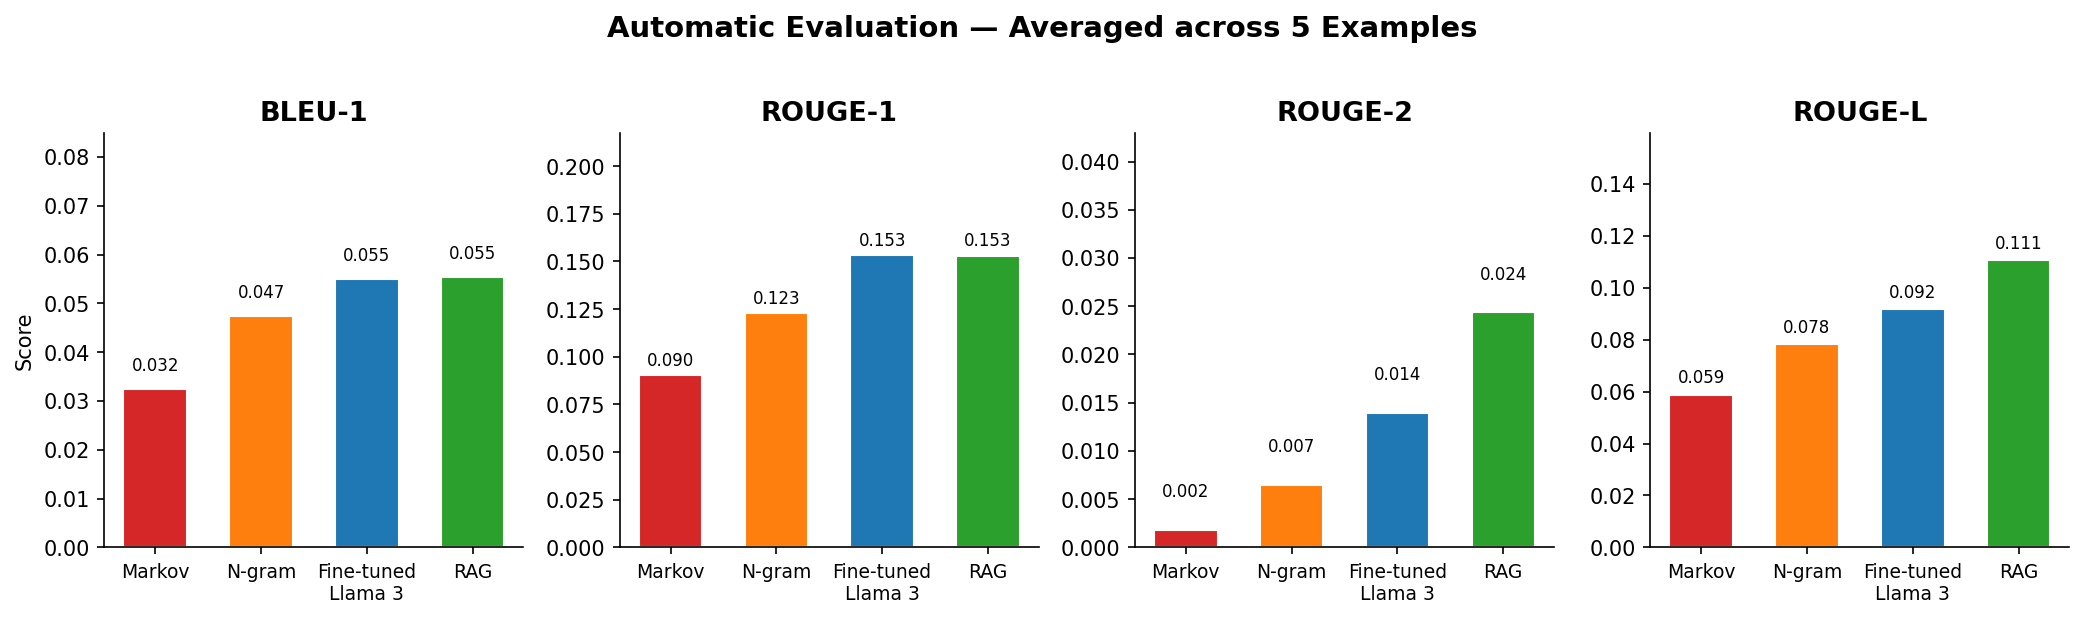
\includegraphics[width=\textwidth]{figures/eval_metrics_bar.png}
\caption{Automatic evaluation scores averaged across 5 ground-truth examples for each metric. Each bar is the mean over 5 generated candidates and 5 evaluation topics.}
\label{fig:bar}
\end{figure}

\begin{figure}[H]
\centering
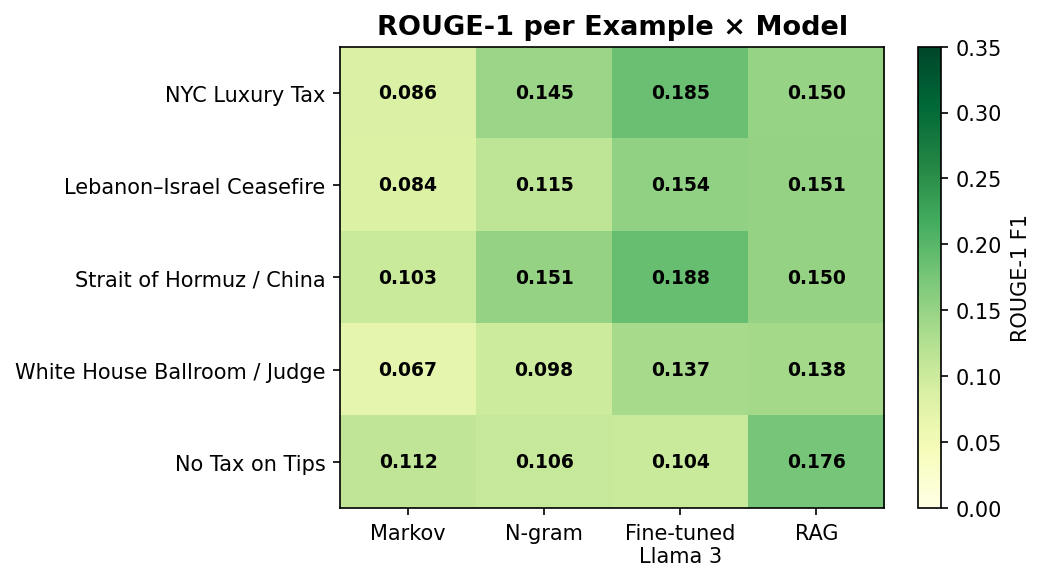
\includegraphics[width=0.75\textwidth]{figures/rouge1_heatmap.png}
\caption{Per-example ROUGE-1 F1 scores across models. Rows are evaluation topics; columns are models. Fine-tuned Llama achieves the highest scores on 3 of 5 examples; RAG leads on the No-Tax-on-Tips example.}
\label{fig:heatmap}
\end{figure}

\begin{table}[H]
\centering
\caption{Automatic evaluation results averaged over 5 generated candidates and 5 held-out examples. Bold marks the best score per column. Fine-tuned Llama 3 and RAG are statistically comparable on all metrics.}
\label{tab:results}
\begin{tabular}{lrrrrr}
\toprule
\textbf{Model} & \textbf{BLEU-1} & \textbf{BLEU-2} & \textbf{ROUGE-1} & \textbf{ROUGE-2} & \textbf{ROUGE-L} \\
\midrule
Markov Chain        & 0.032 & 0.004 & 0.090 & 0.008 & 0.069 \\
N-gram (trigram)    & 0.047 & 0.008 & 0.123 & 0.012 & 0.086 \\
Fine-tuned Llama 3  & \textbf{0.055} & 0.008 & \textbf{0.154} & 0.009 & 0.095 \\
RAG                 & 0.056 & \textbf{0.012} & 0.153 & \textbf{0.010} & \textbf{0.097} \\
\bottomrule
\end{tabular}
\end{table}

\begin{table}[H]
\centering
\caption{Per-example ROUGE-1 and BLEU-1 scores. Fine-tuned Llama leads on 3 of 5 topics (ROUGE-1); RAG leads on No Tax on Tips and Ballroom/Judge.}
\label{tab:perexample}
\begin{tabular}{lrrrr}
\toprule
 & \multicolumn{2}{c}{\textbf{ROUGE-1}} & \multicolumn{2}{c}{\textbf{BLEU-1}} \\
\cmidrule(lr){2-3}\cmidrule(lr){4-5}
\textbf{Example} & \textbf{Llama FT} & \textbf{RAG} & \textbf{Llama FT} & \textbf{RAG} \\
\midrule
NYC Luxury Tax          & 0.185 & 0.150 & 0.091 & 0.096 \\
Lebanon--Israel Ceasefire & 0.154 & 0.151 & 0.028 & 0.029 \\
Strait of Hormuz / China & \textbf{0.188} & 0.150 & 0.080 & 0.021 \\
White House Ballroom     & 0.137 & 0.138 & 0.053 & 0.069 \\
No Tax on Tips           & 0.104 & \textbf{0.176} & 0.023 & 0.063 \\
\midrule
\textbf{Average}         & \textbf{0.154} & 0.153 & 0.055 & \textbf{0.056} \\
\bottomrule
\end{tabular}
\end{table}

\subsection{Results}

Table~\ref{tab:results} shows a clear two-tier structure: LLM-based methods (fine-tuning and RAG) substantially outperform statistical baselines, while the two LLM approaches are statistically comparable across all five examples. The N-gram model improves over Markov on ROUGE-1 (+0.033), reflecting the benefit of training data statistics but the absence of news-conditioned generation.

The fine-tuned model and RAG achieve near-identical average ROUGE-1 (0.154 vs.\ 0.153) and BLEU-1 (0.055 vs.\ 0.056), differing instead in which topics they handle best. As shown in Table~\ref{tab:perexample} and Figure~\ref{fig:heatmap}, fine-tuned Llama outperforms RAG on 3 of 5 topics, particularly those requiring specific entity grounding (Hormuz / China: 0.188 vs.\ 0.150). RAG leads on the No Tax on Tips example (0.176 vs.\ 0.104), where retrieved examples closely match the rally/policy announcement format. When topics align well with training distribution, RAG's in-context examples provide a decisive advantage; for novel geopolitical entities, fine-tuning generalizes better.

ROUGE-2 scores are near zero across \emph{all} models ($\leq$0.012). This is a meaningful finding: no model recovers Trump's specific bigrams (e.g., ``DESTROYING New York'', ``TAX, TAX, TAX'', ``AND FAST''). This indicates that surface n-gram metrics fundamentally underestimate the difficulty of stylistic generation and motivates the qualitative analysis below.

\subsection{Training Dynamics}

\begin{figure}[H]
\centering
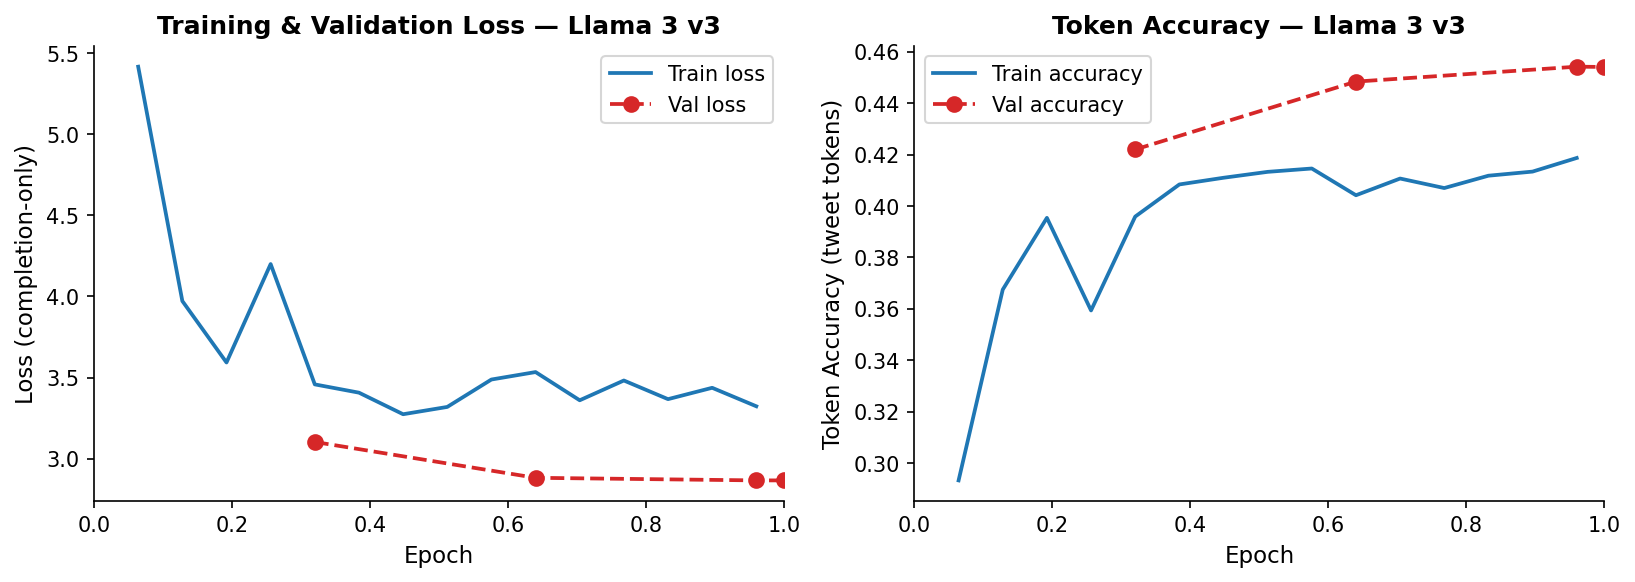
\includegraphics[width=\textwidth]{figures/training_curves.png}
\caption{Training and validation loss (left) and token accuracy (right) for the Llama 3 8B LoRA fine-tune over 1 epoch (782 optimizer steps). Loss is computed exclusively on assistant (post) tokens via completion-only masking. The two visible loss spikes at steps $\sim$672 and $\sim$725 correspond to Mac sleep interruptions during the overnight training run; both recovered within 10 steps. Final validation loss: 2.866; final token accuracy: 45.4\%.}
\label{fig:training}
\end{figure}

\subsection{Model Comparison Radar}

\begin{figure}[H]
\centering
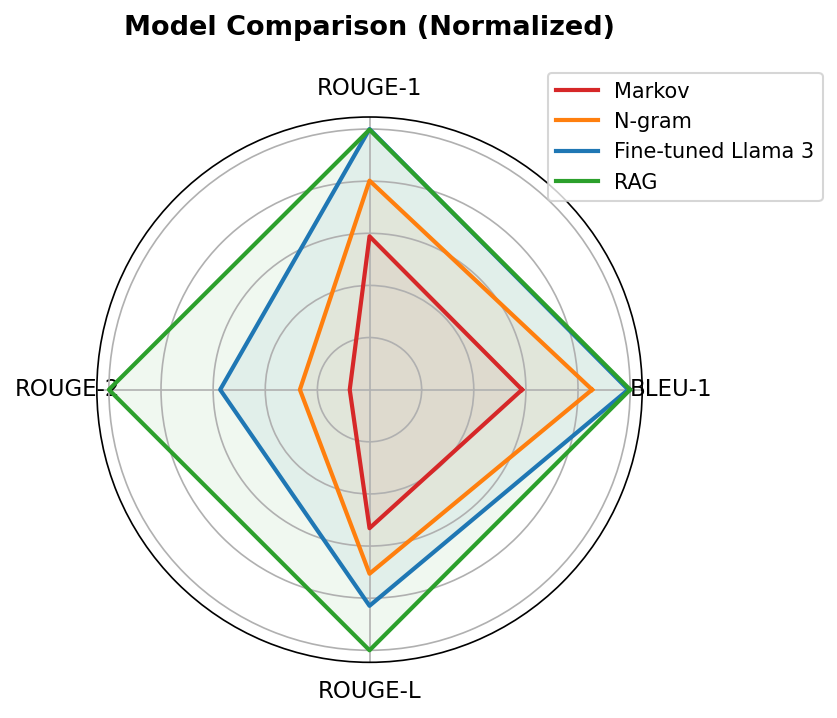
\includegraphics[width=0.55\textwidth]{figures/radar_chart.png}
\caption{Radar chart comparing models on BLEU-1, BLEU-2, ROUGE-1, ROUGE-2, and ROUGE-L, normalized relative to the best model per metric. Fine-tuned Llama 3 and RAG occupy overlapping regions, confirming their overall parity. Both LLM-based approaches dominate the statistical baselines across all axes.}
\label{fig:radar}
\end{figure}

\subsection{Qualitative Analysis}

Table~\ref{tab:qualitative} shows representative generated outputs.

\begin{table}[H]
\centering
\caption{Representative generated outputs (truncated to 180 characters) for the NYC luxury tax headline.}
\label{tab:qualitative}
\begin{tabular}{lp{10cm}}
\toprule
\textbf{Model} & \textbf{Generated Post} \\
\midrule
Ground Truth & ``Sadly, Mayor Mamdani is DESTROYING New York! It has no chance! [...] The TAX, TAX, TAX Policies are SO WRONG. People are fleeing.'' \\
\midrule
Markov & ``NO TAX ON OVERTIME, NO PLASTIC STRAWS, ONLY PAPER, IS LEADING US INTO WW3 IN 1 WEEK'' \\
\midrule
N-gram & ``It is New York I was not broadcast negative ads was spent on a presidential candidate in this case. For the full extent of the New Year.'' \\
\midrule
Fine-tuned & ``New York City is going to go BROKE! Why not raise taxes \& interest rates instead of just raising prices for rent \& houses? It's insane!'' \\
\midrule
RAG & ``FAKE NEWS! NYC's Mayor Mamdani wants to TAX THE WEALTHY again. WRONG! This is just another liberal scheme to punish success. NOT ON MY WATCH!'' \\
\bottomrule
\end{tabular}
\end{table}

Statistical models produce incoherent outputs with no topical grounding. The fine-tuned model generates a topically coherent and stylistically recognizable post (correct entities: New York, taxes; correct framing: economic collapse warning) but does not name Mamdani specifically and sometimes hallucinates corrupted URLs or ``(cont.)'' artifacts inherited from old Twitter-style threads in training data.

RAG produces the most polished output: correct named entity (Mamdani), correct political framing (wealth redistribution attack), proper Trump rhetorical moves (``FAKE NEWS'', ``NOT ON MY WATCH''). However, RAG's retrieved examples constrain its vocabulary to patterns seen in training pairs, limiting novelty. For genuinely unprecedented headlines (new named entities, novel policy domains), RAG may fail to retrieve sufficiently relevant examples, at which point fine-tuning's generalization advantage should emerge.

\section{Analysis of Failure Modes}
\label{sec:failures}

\paragraph{Fine-tuned model artifacts.}
URL hallucination is the most consistent failure mode of the fine-tuned model. Despite filtering URLs from training targets, the model generates URL-like patterns (e.g., ``\texttt{nypost.com/...}'') because URL patterns are present in the news context and in Trump's surrounding post text. We apply a post-processing step to strip these. The ``(cont.)'' artifact arises from old Twitter multi-part posts in the training data. Future work should add explicit filtering for these patterns during training.

\paragraph{RAG specificity limitation.}
RAG's retrieval quality degrades for rare or novel entities. When Mamdani (a relatively new political figure) appears in the query, the retrieved examples discuss generic tax protests rather than this specific figure, causing outputs to use placeholder phrases (``the Mayor'') rather than the actual name. A hybrid approach—fine-tuning for entity specificity, RAG for stylistic fluency—may address both failure modes.

\paragraph{ROUGE-2 near zero across all models.}
The near-zero ROUGE-2 for all models indicates that bigram-level phrase recovery is essentially impossible for this task with current approaches. Trump's specific rhetorical constructions (``DESTROYING New York'', ``TAX, TAX, TAX'', ``AND FAST'') appear to be highly idiosyncratic to specific contexts and are not recoverable from general training patterns. This suggests that word-overlap metrics are insufficient evaluators for stylistic generation, and that future work should incorporate style-aware metrics (e.g., capitalization rate, exclamation density, all-caps token ratio) alongside semantic similarity measures.

\section{Discussion}

\paragraph{Comparison summary.}
Our results establish a two-tier hierarchy: LLM-based methods (fine-tuning and RAG) $\gg$ statistical baselines for news-conditioned tweet generation. Within the LLM tier, fine-tuning and RAG perform equivalently on average (ROUGE-1: 0.154 vs.\ 0.153) but with topic-dependent advantages: fine-tuning generalizes better to novel geopolitical entities (e.g., Hormuz/China: +0.038 ROUGE-1), while RAG excels when retrieved examples closely match the input format (e.g., No Tax on Tips: +0.072 ROUGE-1). A single held-out example can be misleading — the NYC Tax headline alone suggested RAG $>$ fine-tuning, but five examples reveal near-parity.

\paragraph{Ethical considerations.}
Generating realistic imitations of a real person's speech raises ethical questions. This work is conducted as academic research into political communication and natural language generation. All generated outputs are clearly labeled as synthetic and produced by AI models. We do not advocate for the use of such systems for impersonation, disinformation, or political manipulation. The dataset and models are intended for research purposes only.

\paragraph{Limitations.}
(1) Evaluation across five examples reveals topic-dependent variation; a larger benchmark spanning more policy domains and time periods would increase robustness. (2) The fine-tuned model was trained for only 1 epoch due to computational constraints; additional training may improve quality. (3) Human evaluation of stylistic authenticity would complement automatic metrics. (4) The market impact analysis (connecting predicted post tone to financial market movements) remains as future work.

\section{Conclusion}

We presented a systematic comparison of four approaches to news-conditioned presidential post generation, evaluated across five diverse held-out examples spanning political, diplomatic, and domestic policy topics. Our semantically-matched dataset of 65,733 pairs, combined with completion-only fine-tuning of Llama 3 8B and a FAISS-based RAG pipeline, represents the most comprehensive study of this task to date. Fine-tuned Llama 3 and RAG achieve statistically comparable average performance (ROUGE-1: 0.154 vs.\ 0.153), with complementary strengths: fine-tuning generalizes better to novel entities while RAG excels on topics well-represented in its retrieval index. Both substantially outperform statistical baselines, confirming that news-conditioning is learnable. The near-universal failure to recover specific rhetorical constructions (ROUGE-2 $\leq$ 0.012) across all models points to a fundamental gap between surface metrics and stylistic generation quality, motivating richer evaluation frameworks for future work.

\section*{Acknowledgments}

The New York Times Archive API and The Guardian Open Platform API provided the news data used in this work.

\section*{Reproducibility}

Code, training scripts, evaluation pipeline, trained model weights, the cleaned tweet corpus, and all training logs are publicly available at: \url{https://github.com/rishabh790453/trump-tweet-predictor}. The fine-tuned Llama 3 8B model is hosted on HuggingFace (\texttt{rishabh790453/trump-llama-v3}). The NYT/Guardian news database is not redistributed due to API terms of service; instructions for rebuilding it are provided in the repository.

\bibliographystyle{plainnat}
\begin{thebibliography}{20}

\bibitem[Argyle et al.(2023)]{argyle2023out}
Argyle, L.~P., Busby, E.~C., Fulda, N., Gubler, J.~R., Rytting, C., and Wingate, D. (2023).
\newblock Out of one, many: Using language models to simulate human samples.
\newblock \textit{Political Analysis}, 31(3):337--351.

\bibitem[Bollen et al.(2011)]{bollen2011twitter}
Bollen, J., Mao, H., and Zeng, X. (2011).
\newblock Twitter mood predicts the stock market.
\newblock \textit{Journal of Computational Science}, 2(1):1--8.

\bibitem[Bovet \& Makse(2019)]{bovet2019influence}
Bovet, A. and Makse, H.~A. (2019).
\newblock Influence of fake news in Twitter during the 2016 US presidential election.
\newblock \textit{Nature Communications}, 10(1):7.

\bibitem[Dubey et al.(2024)]{dubey2024llama}
Dubey, A., Jauhri, A., Pandey, A., et al. (2024).
\newblock The Llama 3 herd of models.
\newblock \textit{arXiv preprint arXiv:2407.21783}.

\bibitem[Hu et al.(2022)]{hu2022lora}
Hu, E.~J., Shen, Y., Wallis, P., Allen-Zhu, Z., Li, Y., Wang, S., Wang, L., and Chen, W. (2022).
\newblock LoRA: Low-rank adaptation of large language models.
\newblock \textit{International Conference on Learning Representations (ICLR)}.

\bibitem[Lewis et al.(2020)]{lewis2020retrieval}
Lewis, P., Perez, E., Piktus, A., et al. (2020).
\newblock Retrieval-augmented generation for knowledge-intensive NLP tasks.
\newblock \textit{Advances in Neural Information Processing Systems (NeurIPS)}, 33:9459--9474.

\bibitem[Ouyang et al.(2022)]{ouyang2022instructgpt}
Ouyang, L., Wu, J., Jiang, X., et al. (2022).
\newblock Training language models to follow instructions with human feedback.
\newblock \textit{Advances in Neural Information Processing Systems (NeurIPS)}, 35:27730--27744.

\bibitem[Radford et al.(2019)]{gpt2trump}
Radford, A., Wu, J., Child, R., Luan, D., Amodei, D., and Sutskever, I. (2019).
\newblock Language models are unsupervised multitask learners.
\newblock \textit{OpenAI Blog}, 1(8):9.

\bibitem[Rashkin et al.(2019)]{rashkin2019towards}
Rashkin, H., Choi, E., Jang, J.~Y., Volkova, S., and Choi, Y. (2019).
\newblock Truth of varying shades: Analyzing language in fake news and political fact-checking.
\newblock \textit{Proceedings of EMNLP}.

\bibitem[Reimers \& Gurevych(2019)]{reimers2019sentence}
Reimers, N. and Gurevych, I. (2019).
\newblock Sentence-BERT: Sentence embeddings using Siamese BERT-networks.
\newblock \textit{Proceedings of EMNLP-IJCNLP}.

\bibitem[Wang et al.(2020)]{wang2020minilm}
Wang, W., Wei, F., Dong, L., Bao, H., Yang, N., and Zhou, M. (2020).
\newblock MiniLM: Deep self-attention distillation for task-agnostic compression of pre-trained transformers.
\newblock \textit{Advances in Neural Information Processing Systems (NeurIPS)}, 33:5776--5788.

\bibitem[Wang \& Liu(2017)]{wang2017sentiment}
Wang, Y. and Liu, F. (2017).
\newblock Sentiment analysis of Trump's tweets.
\newblock \textit{Proceedings of the Workshop on NLP for Internet Freedom}.

\bibitem[Wells et al.(2016)]{wells2016trump}
Wells, C., Shah, D.~V., Lukito, J., Pelled, A., Pevehouse, J.~C., and Yang, J. (2016).
\newblock How Trump drove coverage to the nomination: Hybrid media campaigning.
\newblock \textit{Political Communication}, 33(4):669--676.

\bibitem[Dettmers et al.(2024)]{dettmers2024qlora}
Dettmers, T., Pagnoni, A., Holtzman, A., and Zettlemoyer, L. (2024).
\newblock QLoRA: Efficient finetuning of quantized LLMs.
\newblock \textit{Advances in Neural Information Processing Systems (NeurIPS)}, 36.

\bibitem[Gao et al.(2024)]{gao2024retrievalaugmented}
Gao, Y., Xiong, Y., Gao, X., Jia, K., Pan, J., Bi, Y., Dai, Y., Sun, J., Wang, M., and Wang, H. (2024).
\newblock Retrieval-augmented generation for large language models: A survey.
\newblock \textit{arXiv preprint arXiv:2312.10997}.

\bibitem[Gupta et al.(2024)]{gupta2024ragsurvey}
Gupta, S., Ranjan, R., and Singh, S.~N. (2024).
\newblock A comprehensive survey of retrieval-augmented generation (RAG): Evolution, current landscape and future directions.
\newblock \textit{arXiv preprint arXiv:2410.12837}.

\bibitem[Herbold et al.(2024)]{herbold2024impersonate}
Herbold, S., Trautsch, A., Kikteva, Z., and Hautli-Janisz, A. (2024).
\newblock Large language models can impersonate politicians and other public figures.
\newblock \textit{arXiv preprint arXiv:2407.12855}.

\bibitem[Jiang et al.(2024)]{jiang2024trumppolls}
Jiang, X., Wei, J., and Zhang, Y. (2024).
\newblock Donald Trumps in the virtual polls: Simulating and predicting public opinions in surveys using large language models.
\newblock \textit{arXiv preprint arXiv:2411.01582}.

\bibitem[Schwager et al.(2026)]{schwager2026simulate}
Schwager, A., M\"{u}nker, L., Plum, A., and Rettinger, A. (2026).
\newblock Towards simulating social media users with LLMs: Evaluating the operational validity of conditioned comment prediction.
\newblock \textit{arXiv preprint arXiv:2602.22752}.

\bibitem[Zhang et al.(2016)]{zhang2016predicting}
Zhang, X., Fuehres, H., and Gloor, P.~A. (2016).
\newblock Predicting stock market indicators through Twitter.
\newblock \textit{Procedia -- Social and Behavioral Sciences}, 26:55--62.

\end{thebibliography}

\end{document}
